\begin{appendices}
%\appendix
\renewcommand\thefigure{\thesection.\arabic{figure}} 
\setcounter{figure}{0}

%\section*{Appendices}
%\addcontentsline{toc}{chapter}{Appendices}
\renewcommand{\thesection}{\Alph{section}}

\definecolor{codegreen}{rgb}{0,0.6,0}
\definecolor{codegray}{rgb}{0.5,0.5,0.5}
\definecolor{codepurple}{rgb}{0.58,0,0.82}
\definecolor{backcolour}{rgb}{0.95,0.95,0.92}
\definecolor{deepred}{rgb}{0.6,0,0}
 
\lstdefinestyle{mystyle}{
    backgroundcolor=\color{backcolour},   
    commentstyle=\color{codegreen},
    keywordstyle=\color{blue},
    numberstyle=\tiny\color{codegray},
    stringstyle=\color{codepurple},
    basicstyle=\footnotesize,
    breakatwhitespace=false,         
    breaklines=true,                 
    captionpos=b,                    
    keepspaces=true,                 
    numbers=left,                    
    numbersep=5pt,                  
    showspaces=false,                
    showstringspaces=false,
    showtabs=false,                  
    tabsize=2
}
 
\lstset{style=mystyle}


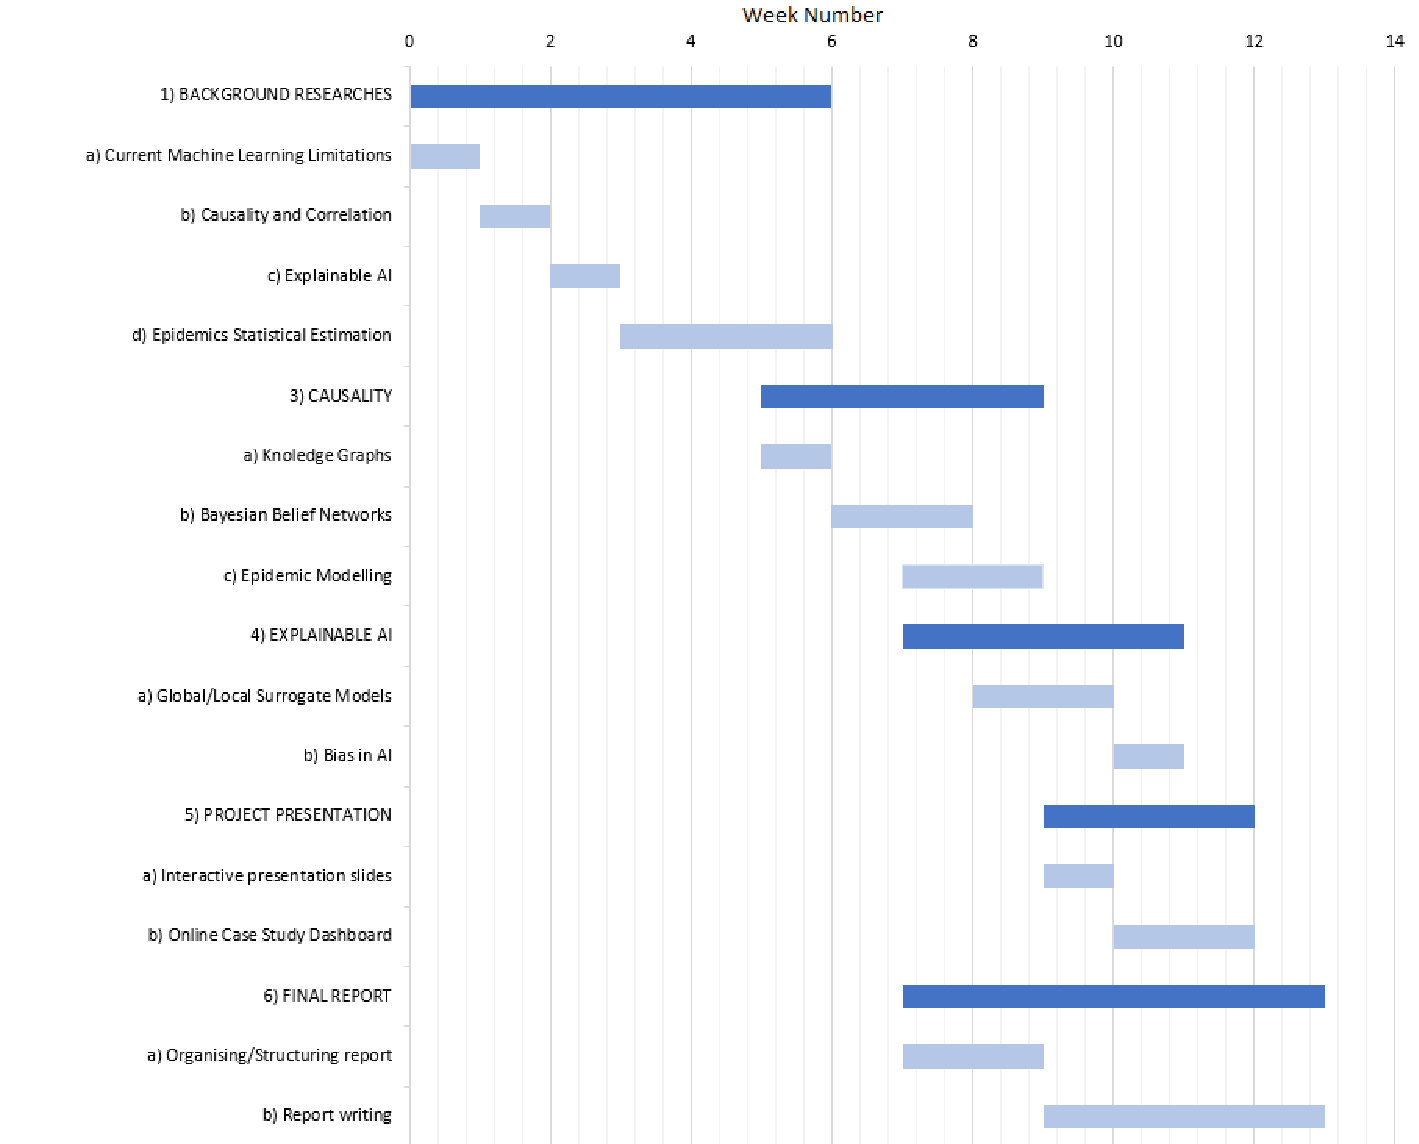
\includepdf[pages=-,pagecommand={\section{Project Management}\label{man}\null\vfill\captionof{figure}{Planned Gantt Chart}},noautoscale=true,offset=0 -10, scale=0.70]{images/gann.pdf}

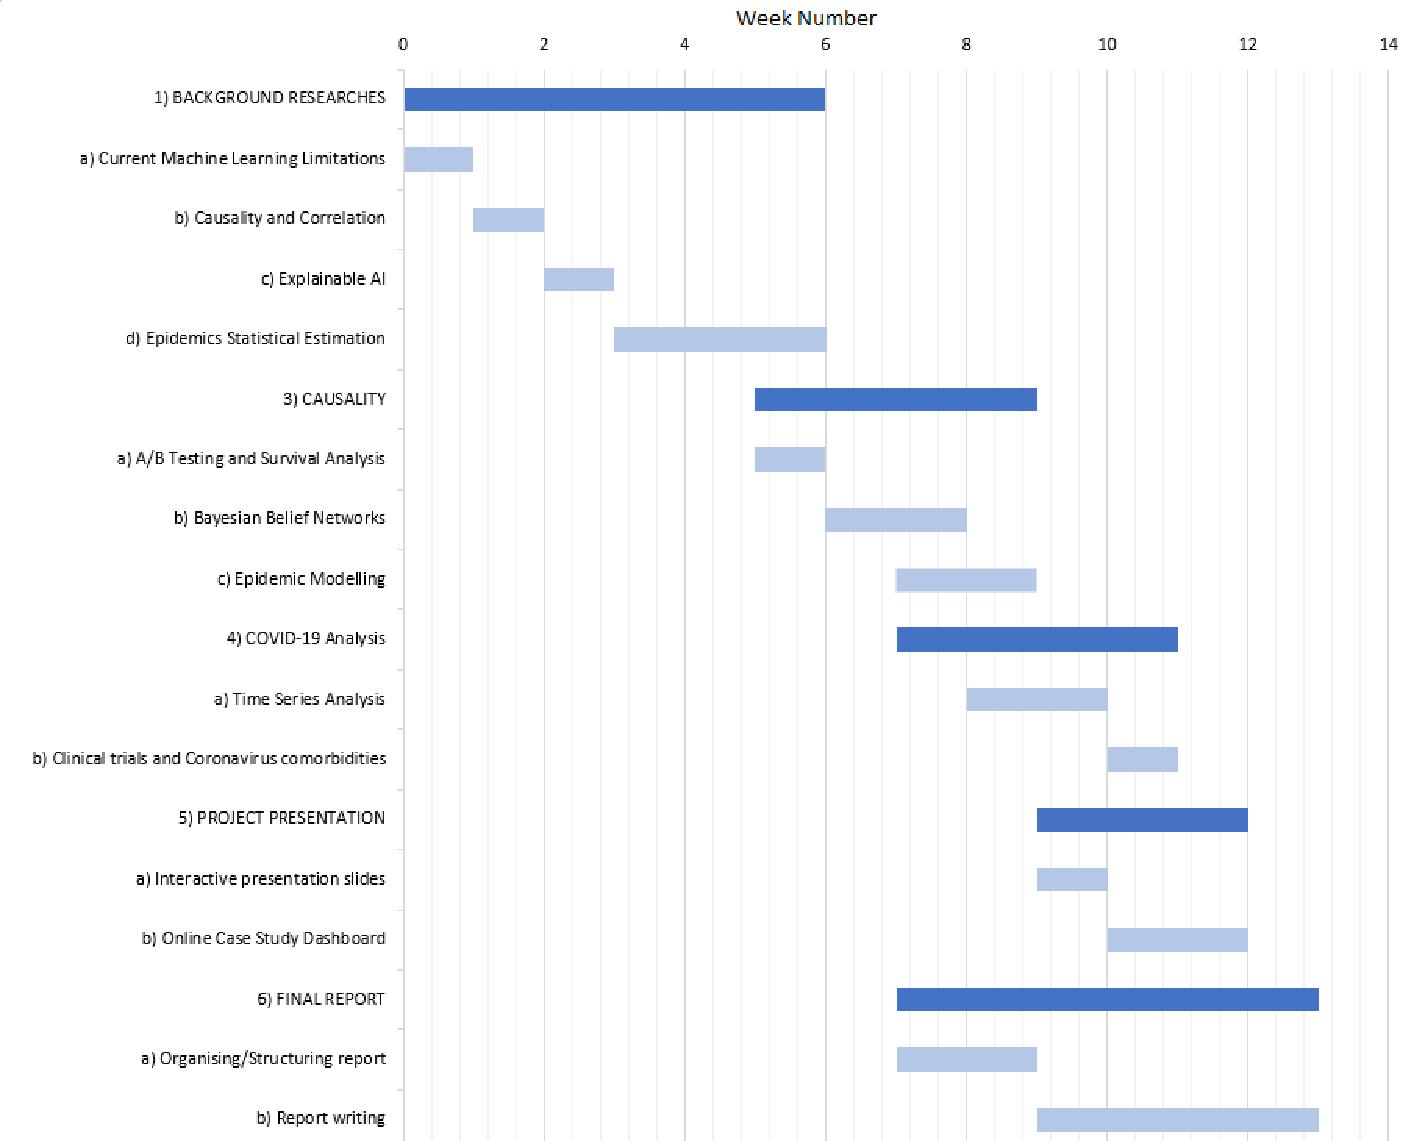
\includepdf[pages=-,pagecommand={\null\vfill\captionof{figure}{Actual Gantt Chart}},noautoscale=true,offset=0 -10, scale=0.7]{images/actual_gannt.pdf}

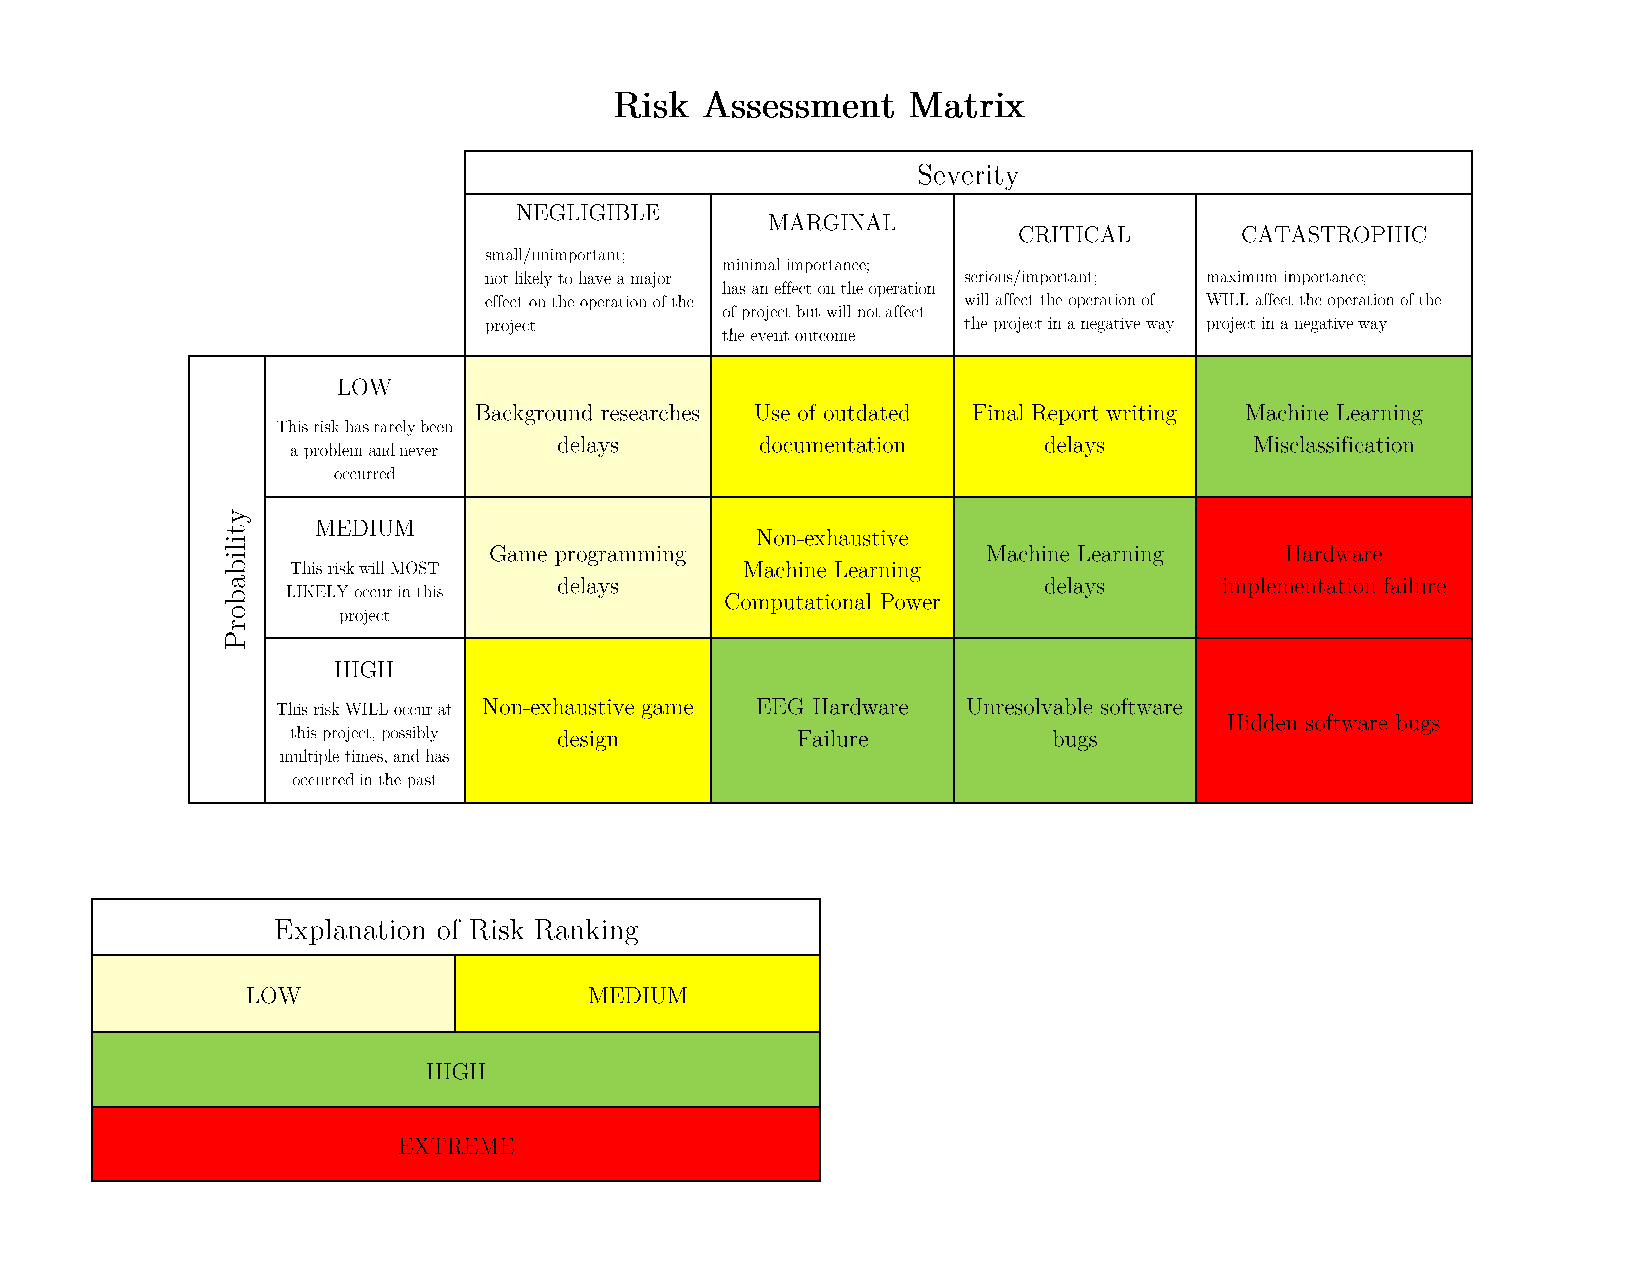
\includepdf[pages=-,pagecommand={\null\vfill\captionof{figure}{Risk Assesment Matrix}},noautoscale=true,offset=0 -10, scale=0.7]{images/Management.pdf}

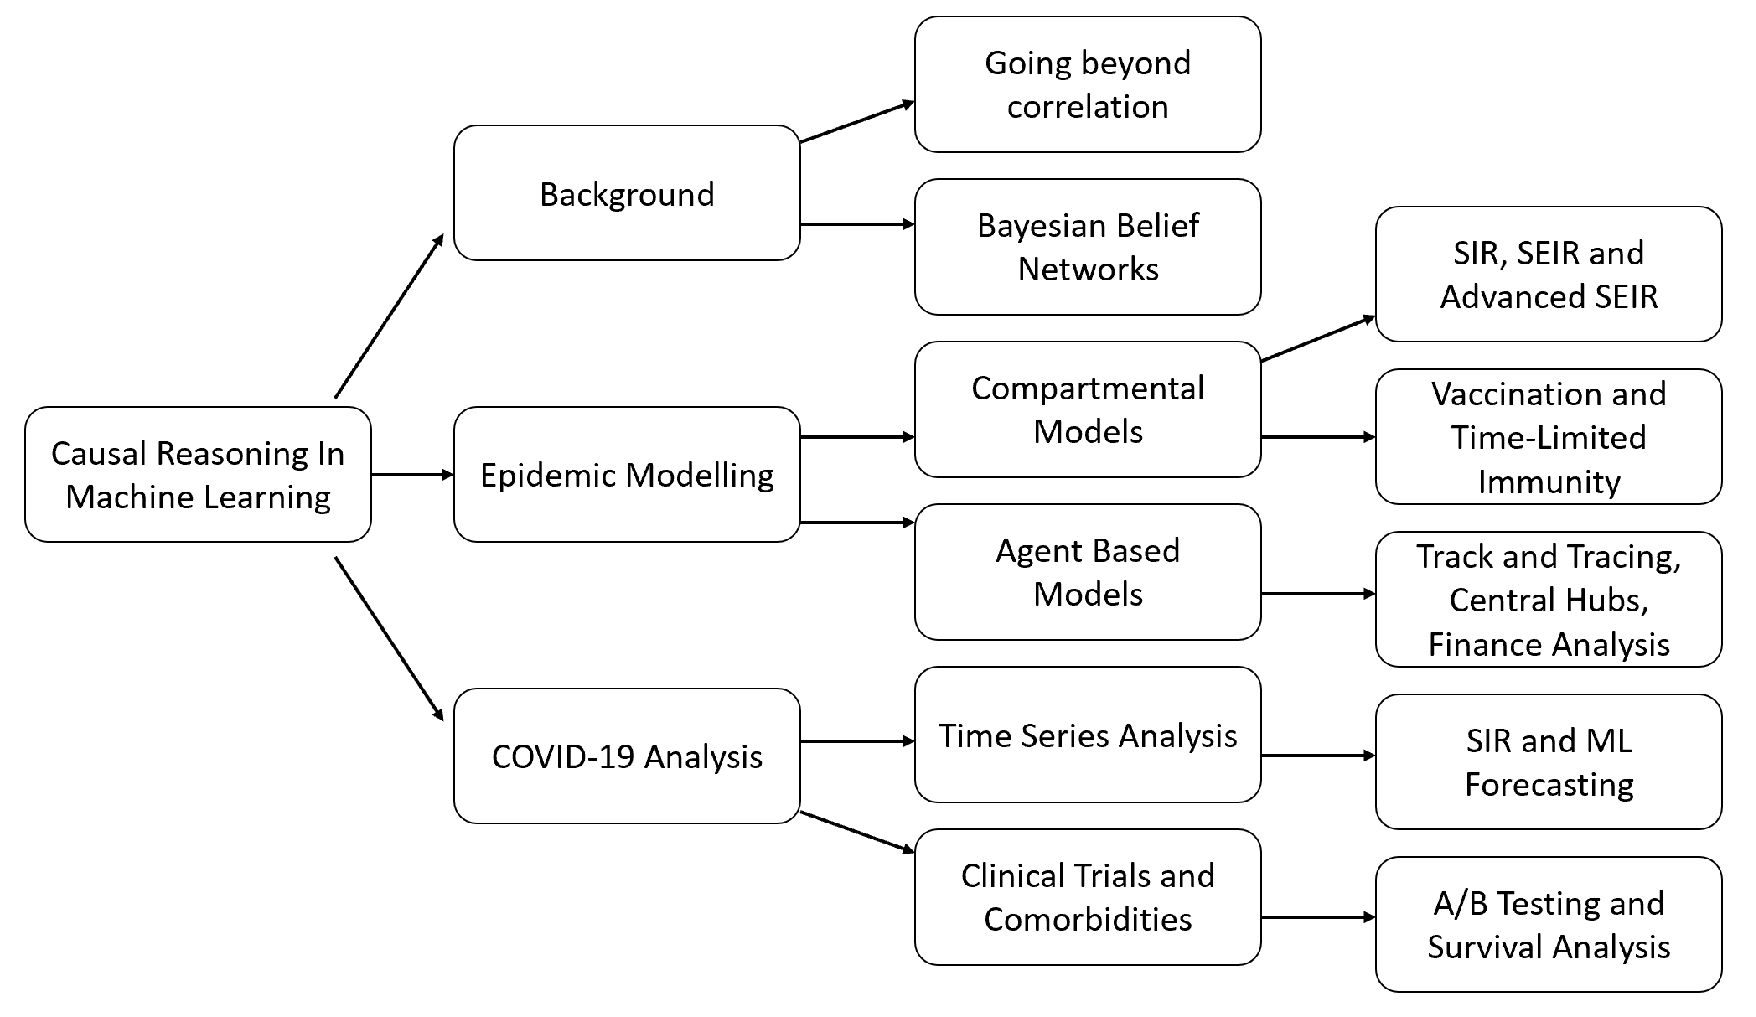
\includepdf[pages=-,pagecommand={\null\vfill\captionof{figure}{Work Breakdown Structure}},noautoscale=true,offset=0 -10, scale=0.6,angle=90]{images/WBS.pdf}

\section{Power Predictive Score (PPS)}
\label{pps}

During the last few years, different approaches have been taken in order to try to overcome correlation limitations. This research focus led then to the development of the "Causality Revolution" and alternative metrics to correlation such as the \textbf{Predictive Power Score (PPS)} \cite{ppc}.

Typical correlation analysis is able to tell us if there is a linear relationship between different variables by returning a score between -1 (e.g. if one variable increase in values, the other decreases) and 1 (e.g. if one variable increases in value, the other one will follow a similar trend). Although, correlation is not able to identify any non-linear relationship and is not able to handle non-numeric data. In the case of categorical data, this could potentially be converted into numerical data by using for example One Hot Encoding or Word Embedding techniques but would most likely lead to an increase of the dataset dimensionality in order to achieve good results. Finally, correlation might not be able to understand if relationships between the different columns are symmetric or asymmetric.

In Figure \ref{corr_t}, is available a summary of some examples of correlation trends and limitations.

\vspace{-0.1cm}
\begin{figure}[ht!]%
    \centering
    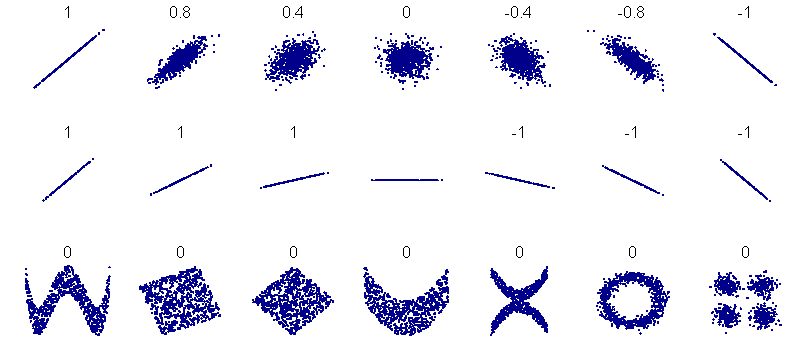
\includegraphics[width=0.85\linewidth]{latex/images/corr.pdf}
    % 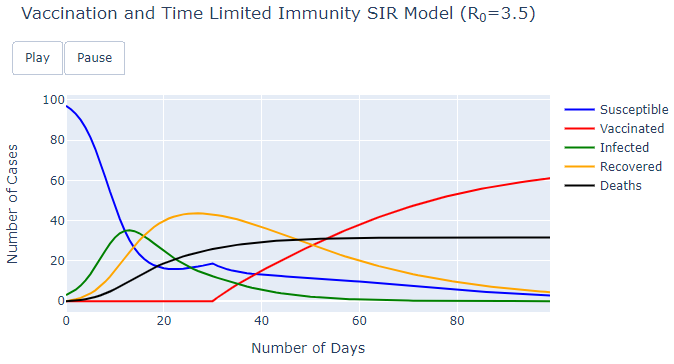
\includegraphics[width=13cm]{latex/images/vacc.PNG}%
    \vspace{-0.2cm}
    \caption{Correlation Trends (Image reproduced from \cite{corr_trends})}
    \label{corr_t}
\end{figure}
\vspace{-0.5cm}

The predictive power score has been ideated in order to try to overcome the presented correlation limitations. One possible way to calculate the PPS is to train a Cross-Validated Decision Tree model on one feature and consider the other feature we want to consider as our label. We can then evaluate the model using an appropriate evaluation metric and then normalise the score by comparing it with the score obtained by a naive predictor. A possible set-up for a PPS calculation is shown in Table \ref{setup}.

{
\begin{table}[h!]
\centering
\begin{tabular}{l|l|c|c|c}
\multicolumn{2}{c}{}&\multicolumn{2}{c}{}&\\
\cline{3-4}
\multicolumn{2}{c|}{}&Numeric Data &Categorical Data &\multicolumn{1}{c}{}\\
\cline{2-4}
\multirow{}{}{}& ML Model & Decision Tree Regressor & Decision Tree Classifier & \\
\cline{2-4}
& Evaluation Metric & Mean Absolute Error & Weighted F1 Score & \\
\cline{2-4}
& Naive Predictor & Predict median value & Predict most common class & \\
\cline{2-4}
% \multicolumn{1}{c}{} & \multicolumn{1}{c}{} & \multicolumn{1}{c}{} & \multicolumn{1}{c}{} & \multicolumn{1}{c}{}\\
\end{tabular}
% \vspace{-0.7cm}
\caption{Predictive Power Score Set-up}
\label{setup}
\end{table}
}

Where the Mean Absolute Error (MAE) and F1 score can be defined as:

\useshortskip
\begin{align}
\ F1 = 2 \times \dfrac{precision \times recall}{precision + recall}
\ MAE = \dfrac{1}{n}\sum_{i=1}^{n}\abs{x_{i} - x}
\end{align}
\useshortskip

The result from the evaluation metric can then be normalised by comparing it with the results from the naive predictor. In the case of the F1 Score, one is going to be considered our upper limit and the naive predictor score as our lower limit.

\useshortskip
\begin{align}
\ PPS = \dfrac{Decision\:Tree\:(F1) - Naive\:Predictor\:(F1)}{1 - Naive\:Predictor\:(F1)}
\end{align}
\useshortskip

A similar formula could then be calculated for the MAE case, but zero should be considered as our lower limit (in this case, lower scores are considered as better).

\useshortskip
\begin{align}
\ PPS = 1 - \dfrac{Decision\:Tree\:(MAE)}{Naive\:Predictor\:(MAE)}
\end{align}
\useshortskip

Following this procedure, we would then have a PPS score between 0 (no relationship) and 1 (perfect relationship) able to capture either linear/non-linear relationships and to work with either numerical or categorical data. 

As a simple demonstration of the PPS score, there is shown in Figure \ref{pps_ex} a noisy cosine function. In this example, the X axis has been realised by creating a uniform range between 0 and 1000, while the Y axis has been created by passing the respective X value in a cosine function and adding some small noise on the result. In this way, it is designed a clear non-linear dependence between X and Y. 

Calculating the correlation between the two features would then lead to a result equal to zero (from either points of view). Using instead the PPS would then lead as expected to a score of 0.737 of X respect to Y and of 0 for Y respect to X. 

% \vspace{-0.1cm}
\begin{figure}[ht!]%
    \centering
    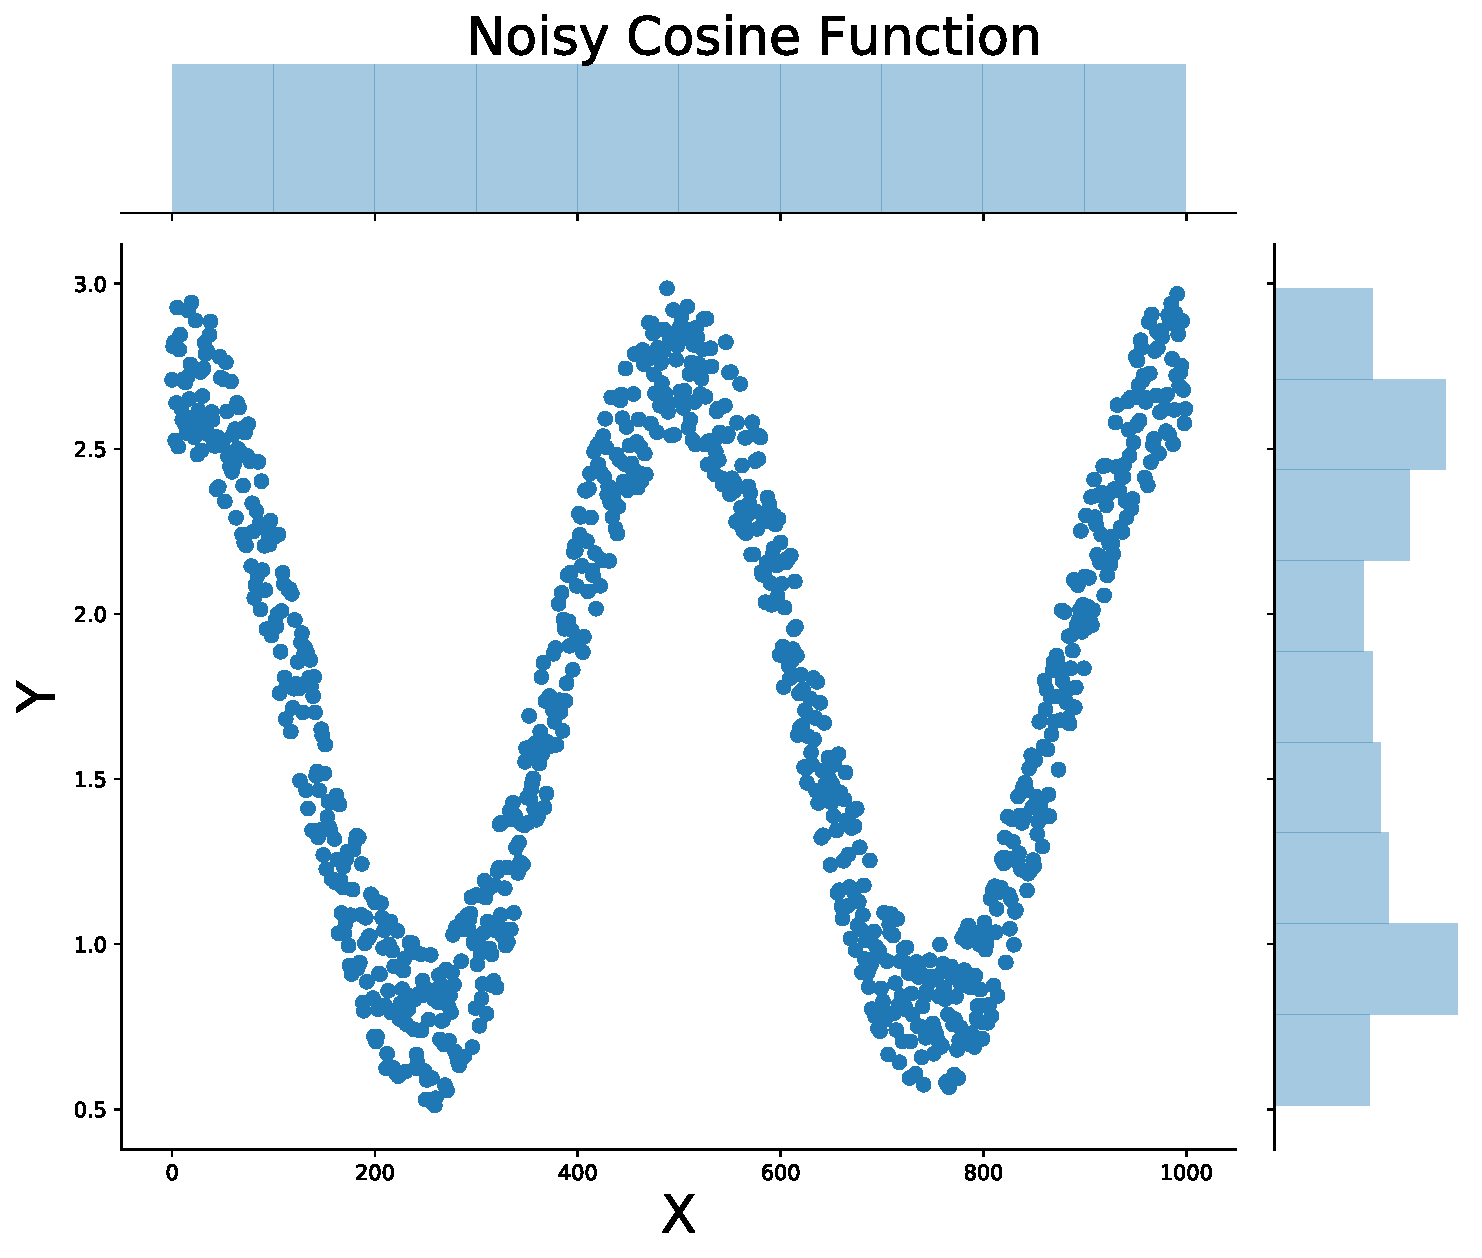
\includegraphics[width=0.45\linewidth]{latex/images/pps_ex.pdf}
    % 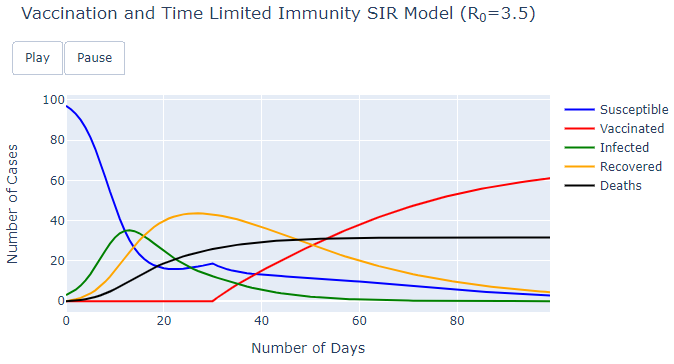
\includegraphics[width=13cm]{latex/images/vacc.PNG}%
    \vspace{-0.2cm}
    \caption{PPS Score Example}
    \label{pps_ex}
\end{figure}
% \vspace{-0.1cm}

The Predictive Power Score is just one of the different approaches which can be taken in order to go beyond correlation traditional limitations, other examples are: Causality, relative entropy and Granger techniques.

\clearpage

\section{Logistic/Exponential Curve Fitting}
\label{exp_fit}

For a logistic curve at the turning point: 

\useshortskip
\begin{align}
\ Slope = Growth\:Factor/2 \Rightarrow\quad Doubling\:Time\:(DT) = \dfrac{ln(2)}{Growth \:Factor/2}
\end{align}
\useshortskip

Instead, for an exponential curve:

\useshortskip
\begin{align}
\ Slope = Growth\:Factor \Rightarrow\quad Doubling\:Time\:(DT) = \dfrac{ln(2)}{Growth\:Factor}
\end{align}
\useshortskip

A worked out example with the results from the top three countries with the most number of Coronavirus Cases as of the end of June 2020, is available below. From this example, we can easily see how well our data resembles a logistic/exponential curve (using the $R^{2}$ score to quantify the mismatch) and what's the predicted time for the number of cases to double given the current trends.

\begin{figure}[ht!]%
    \centering
    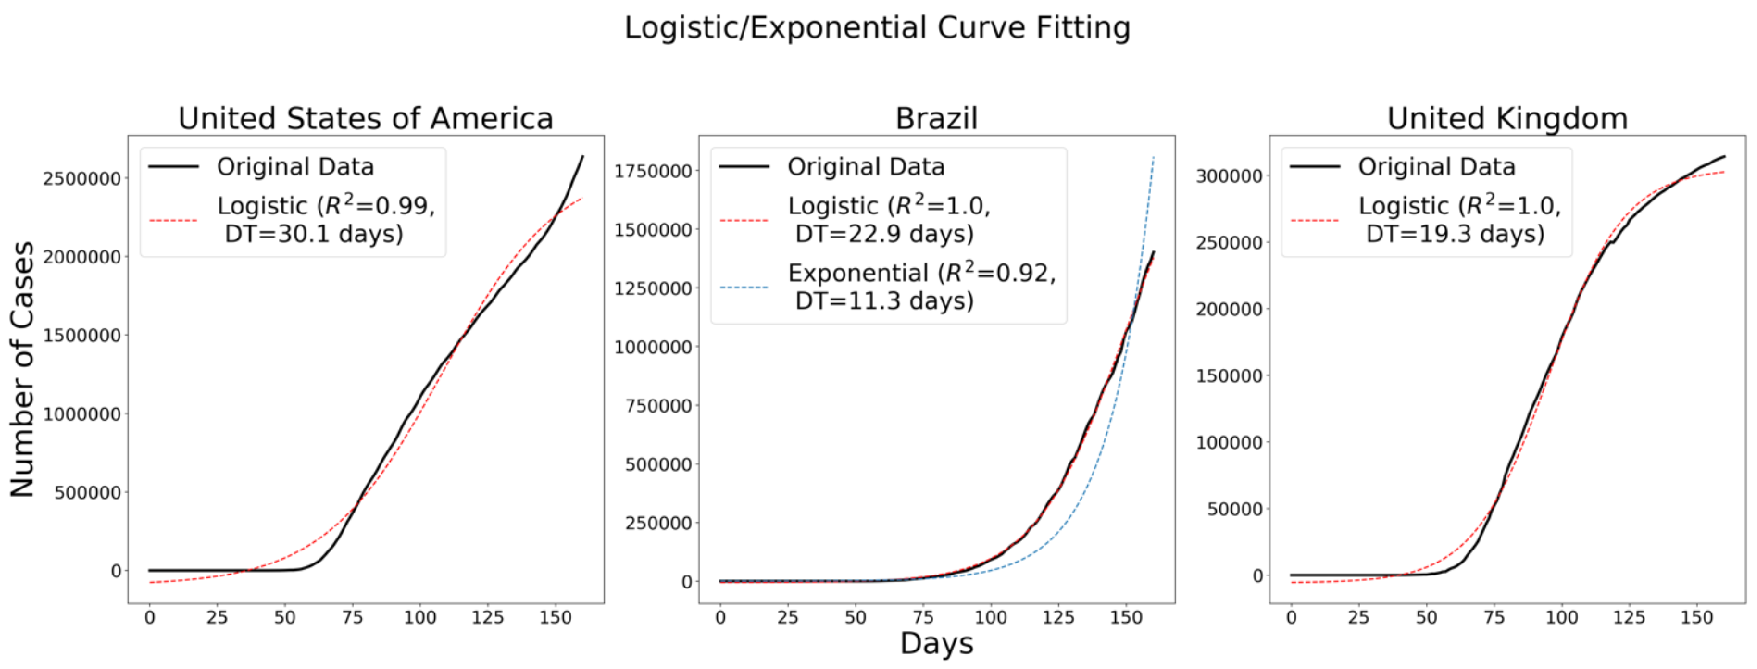
\includegraphics[width=1\linewidth]{latex/images/fitting.pdf}
    % 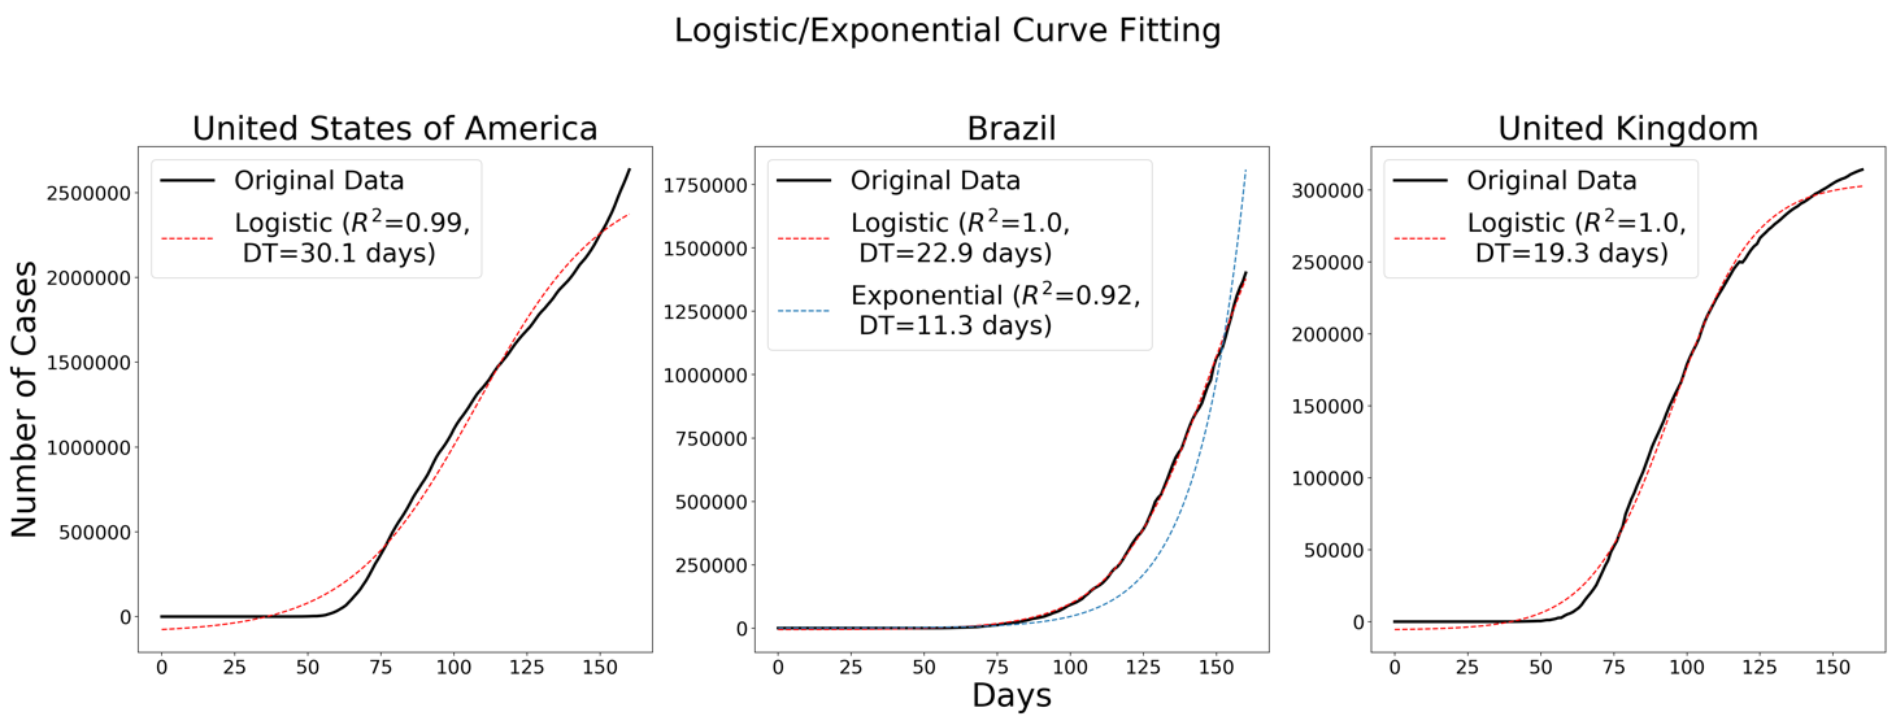
\includegraphics[width=15.5cm]{latex/images/fitting.PNG}%
    \caption{Curve Fitting}
\end{figure}

\clearpage

\section{Project Demonstration}
\label{dem}

Two of the main functionalities of the created secondary GitHub pages website are a Reveal.js online presentation of the whole project and a D3.js scroller page created for interactively presenting and explaining different concepts of this research project. In Figure \ref{revealjs_ex}, there is available an example of part of the created Reveal.js presentation.

\begin{figure}[ht!]%
    \centering
    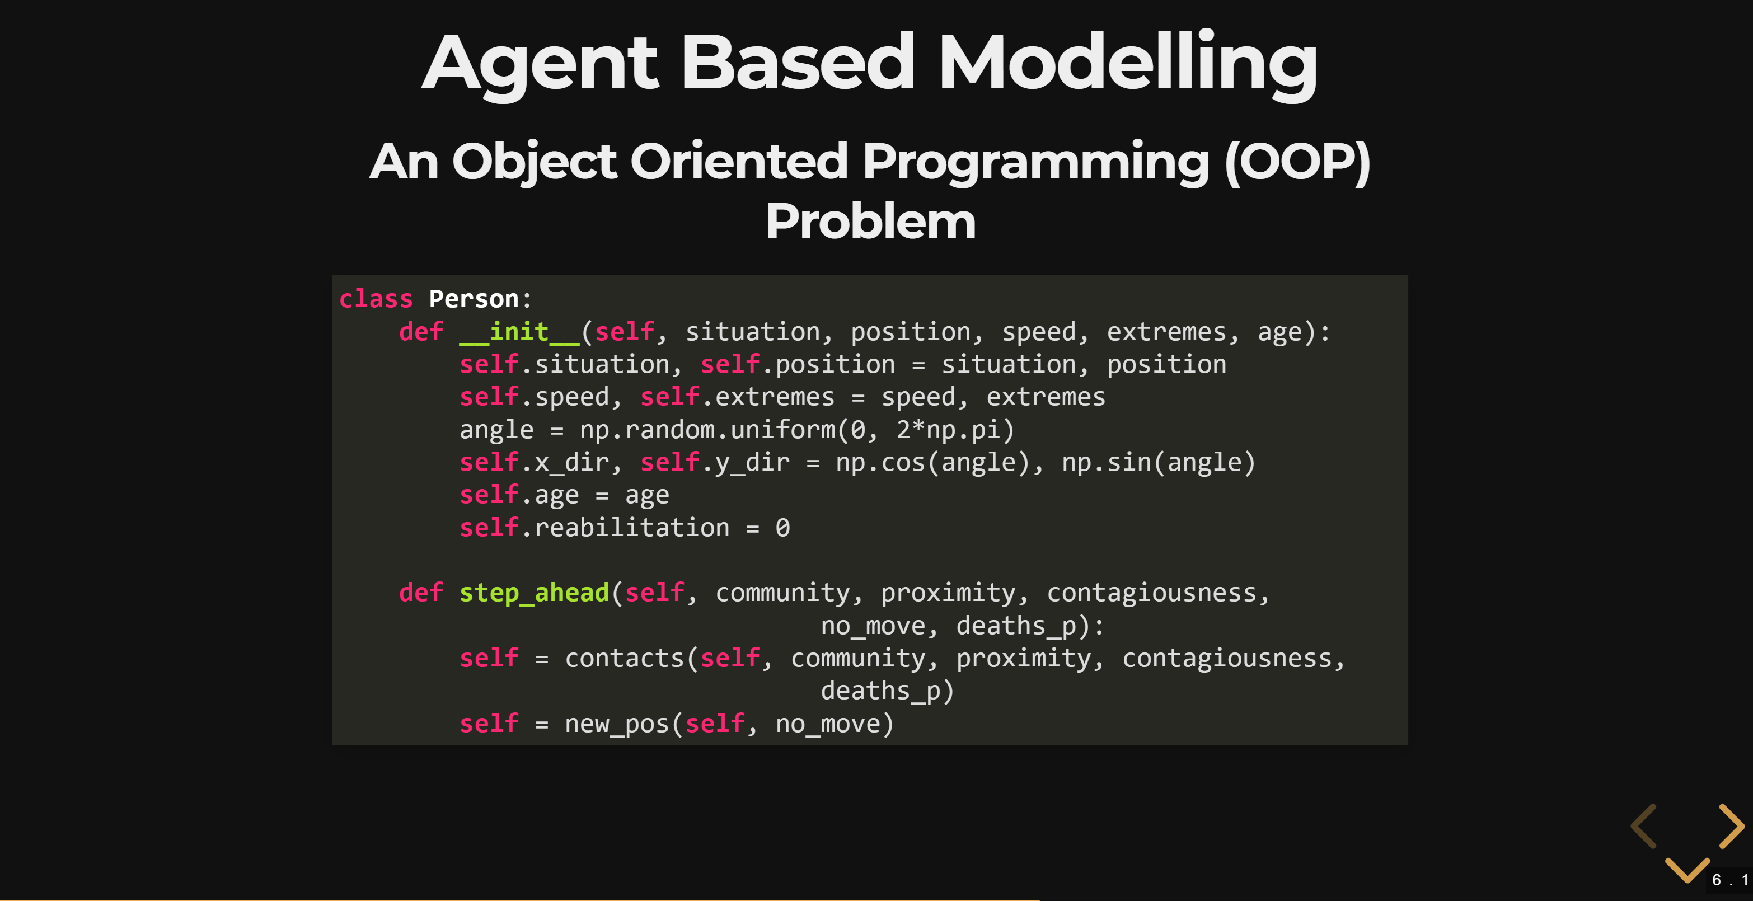
\includegraphics[width=1\linewidth]{latex/images/demo1.pdf}
    % 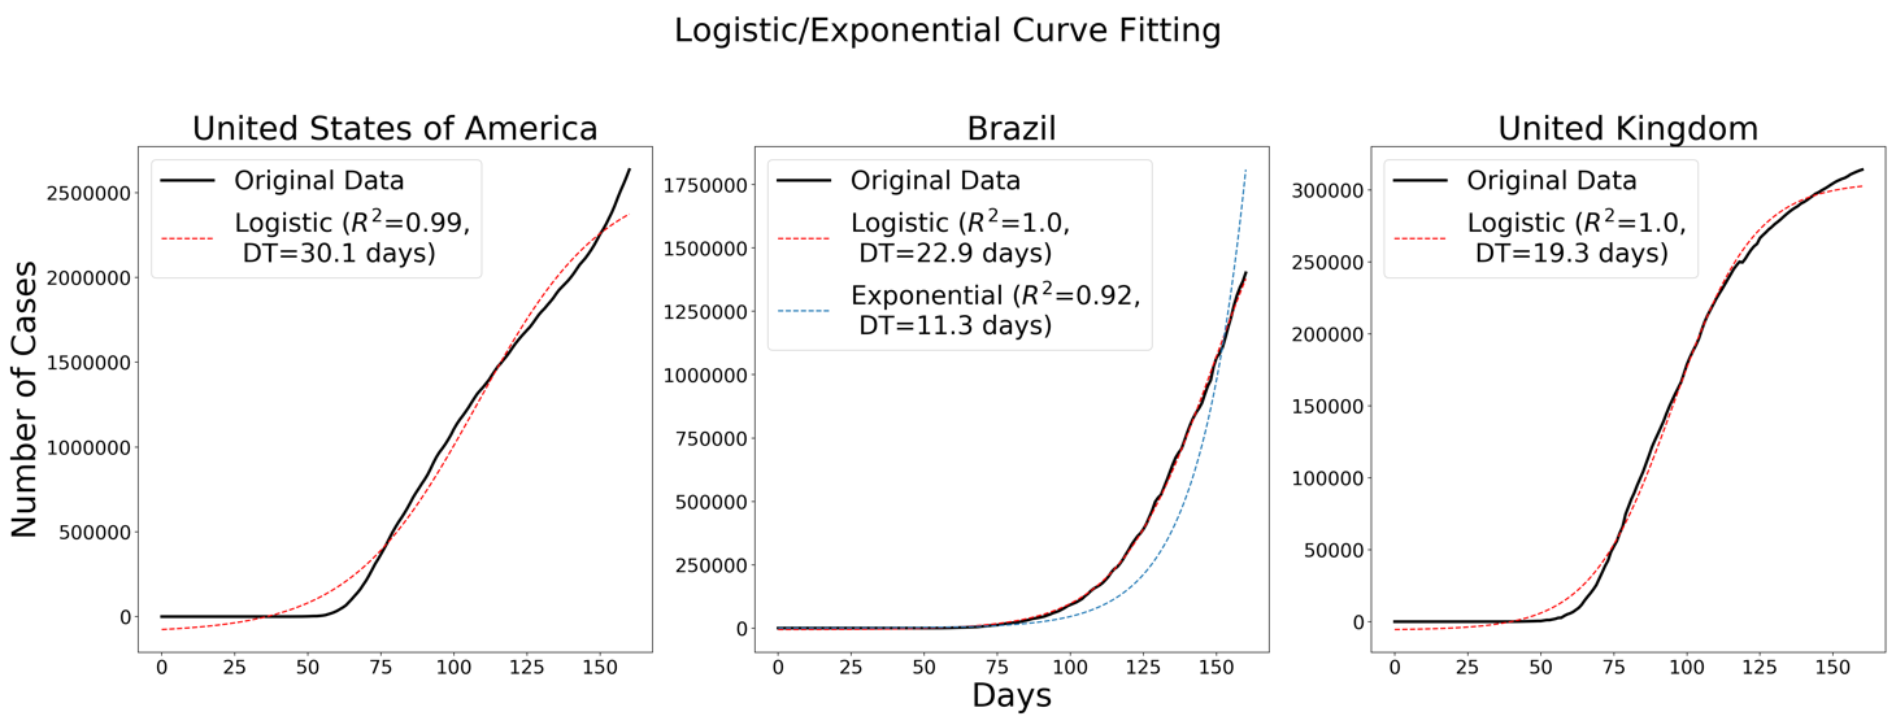
\includegraphics[width=15.5cm]{latex/images/fitting.PNG}%
    \caption{Reveal.js Presentation}
    \label{revealjs_ex}
\end{figure}
\vspace{-0.3cm}
In Figure \ref{d3js_ex}, there is instead shown the first section of the created D3.js story-telling narrative.

\begin{figure}[ht!]%
    \centering
    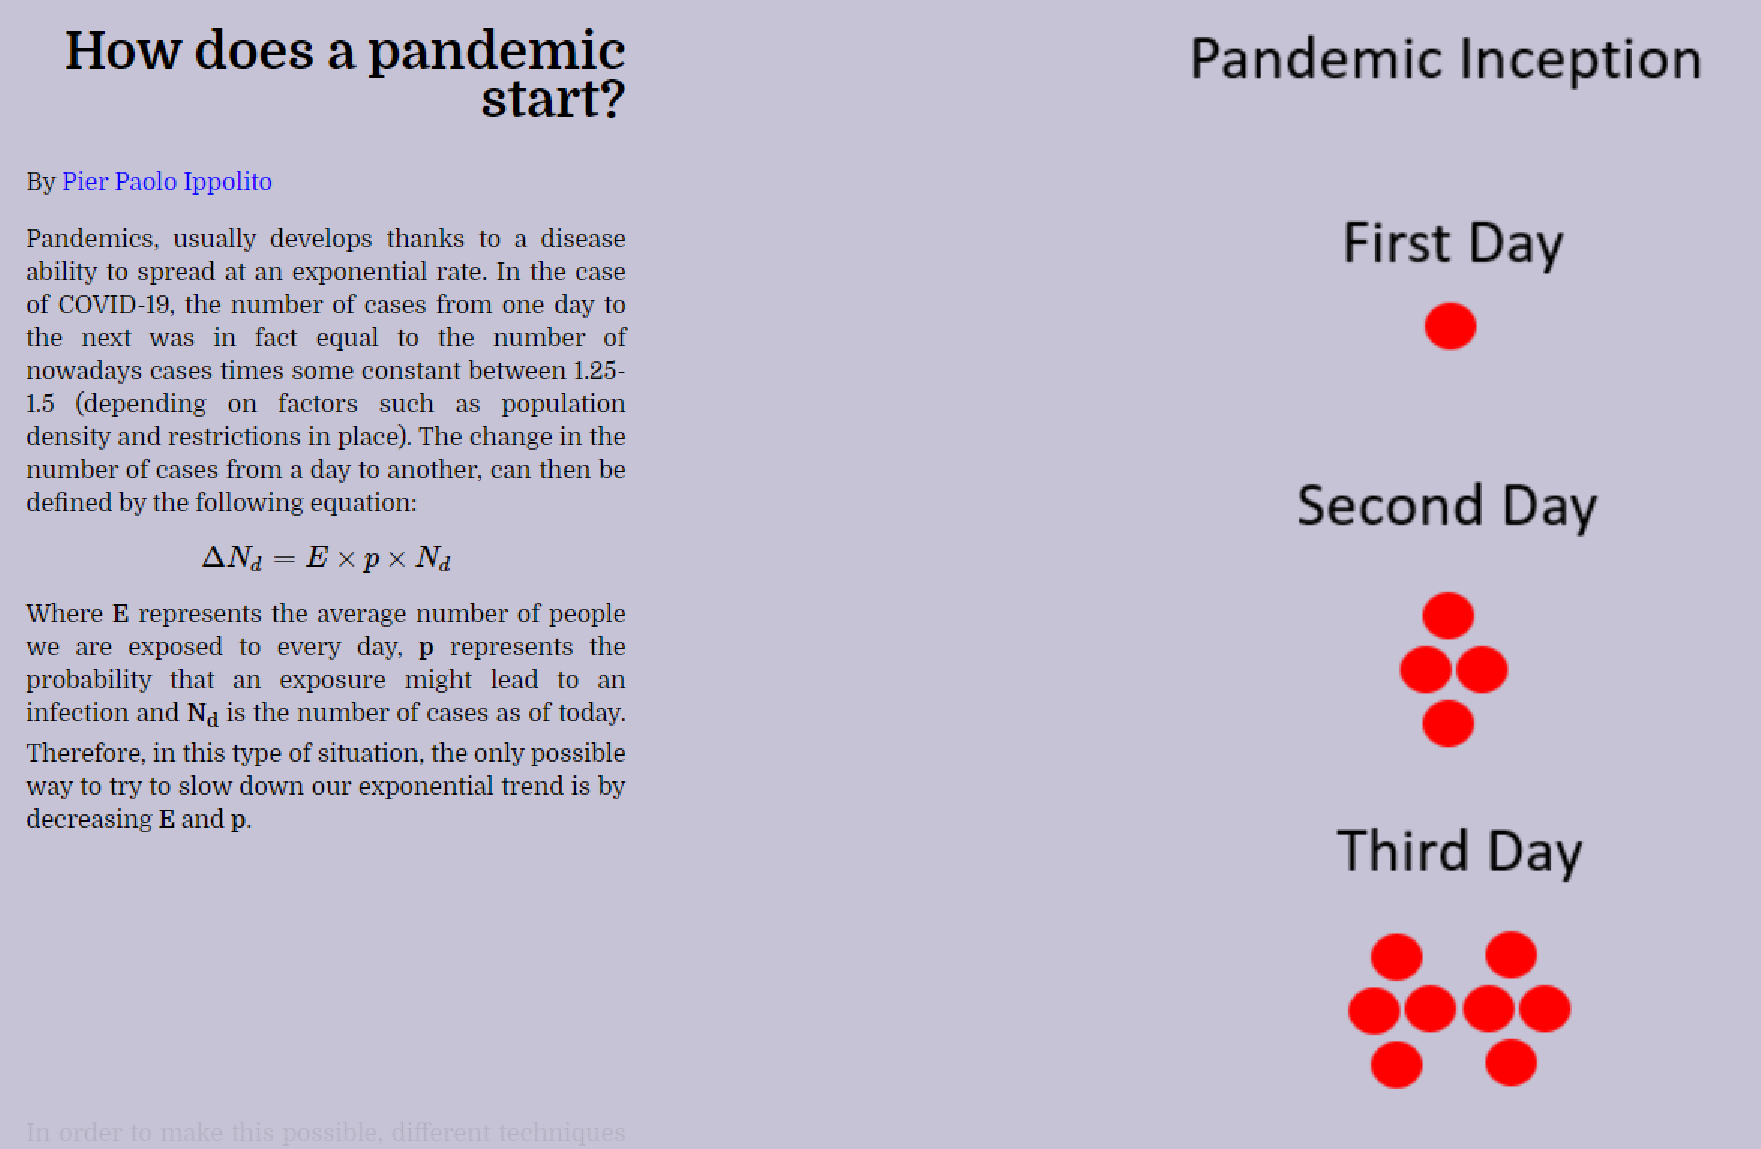
\includegraphics[width=0.8\linewidth]{latex/images/d3js_demo.pdf}
    % 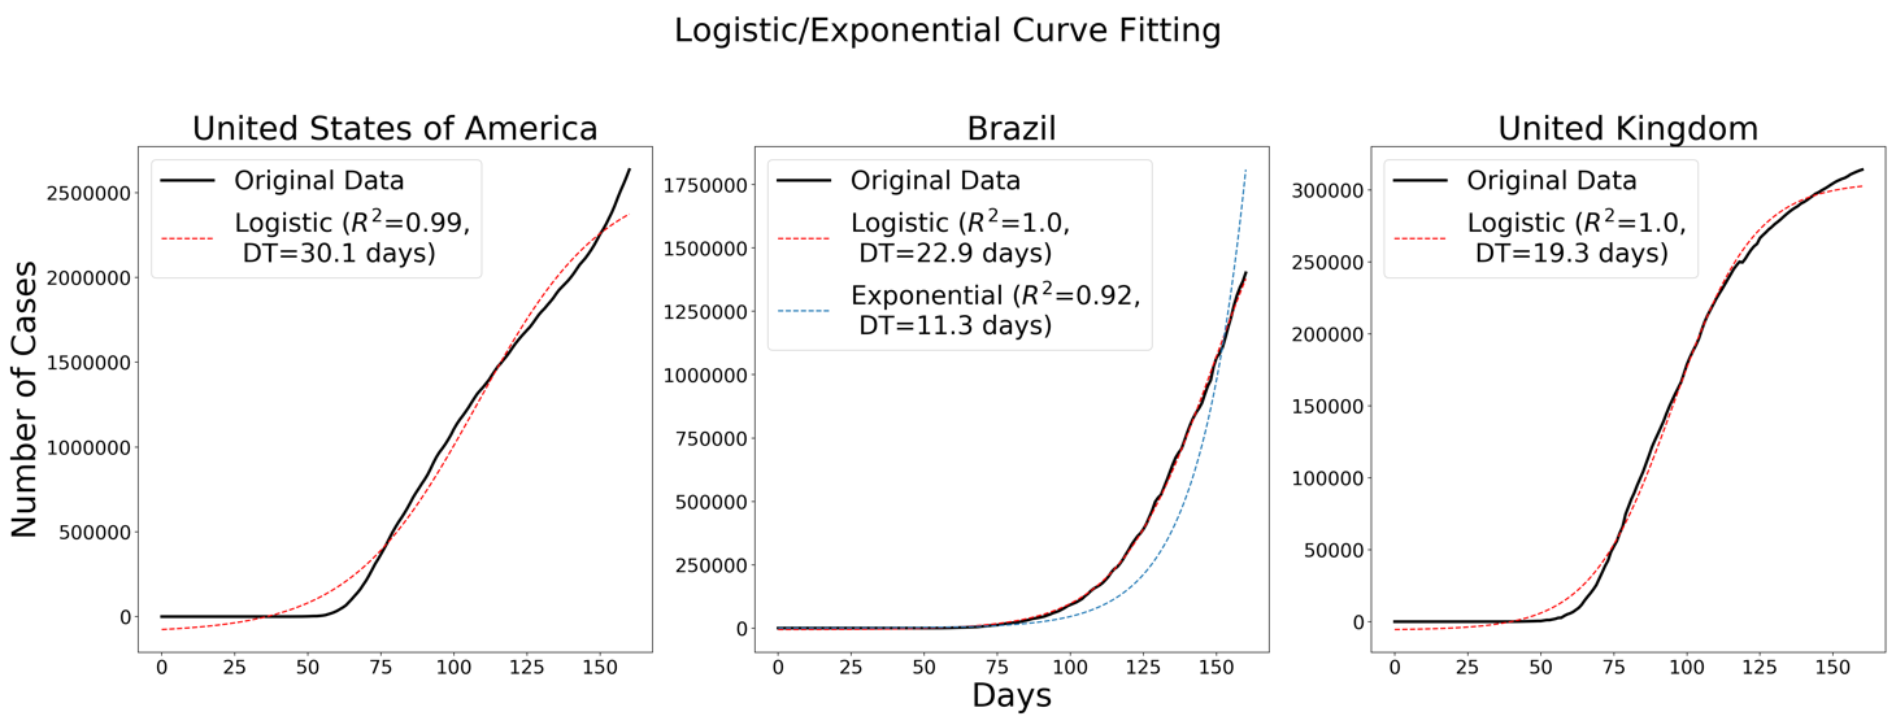
\includegraphics[width=15.5cm]{latex/images/fitting.PNG}%
    \caption{D3.js Scroller}
    \label{d3js_ex}
\end{figure}

\newpage
\section{Compartmental Models Causal Diagrams}
\label{causal_comp}

In this Appendix there are available the Causal Diagrams of the epidemic compartmental models introduced in Section \ref{sir_sec}.

The SIR and SEIR models can be described as shown in Figure \ref{cd11} using a causal chain.

\begin{figure}[ht!]%
    \centering
    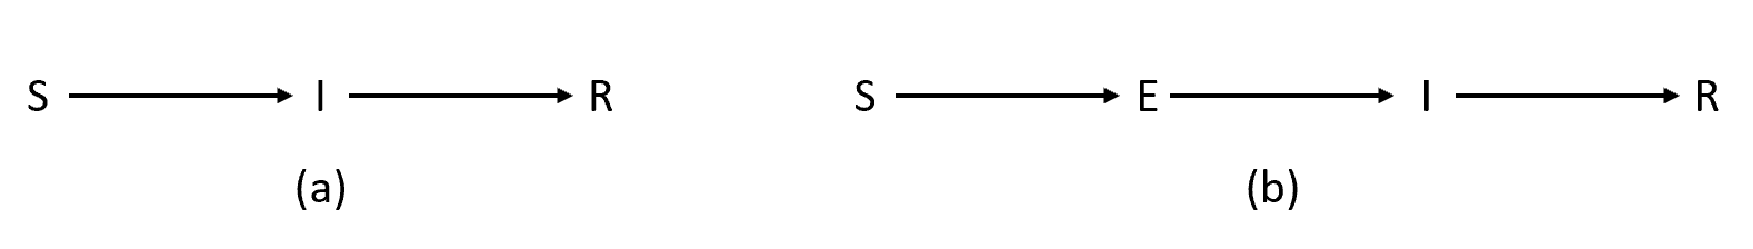
\includegraphics[width=0.9\linewidth]{latex/images/caus_eq.pdf}
    % 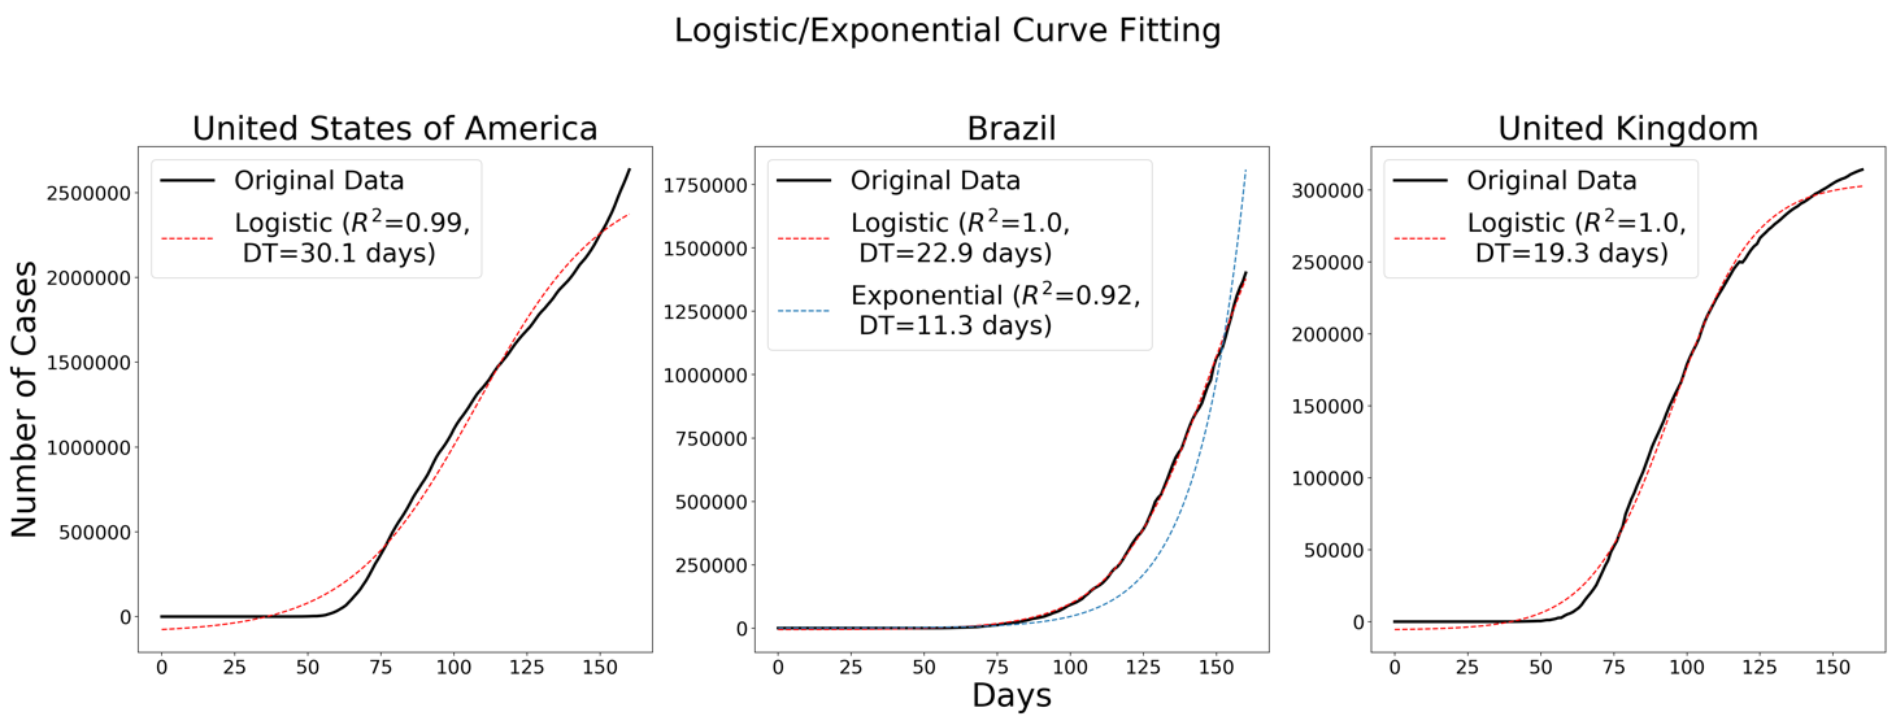
\includegraphics[width=15.5cm]{latex/images/fitting.PNG}%
    \caption{SIR and SEIR}
    \label{cd11}
\end{figure}

The SEIR model including also a deaths compartment can instead be described by a chain followed by a fork junction. Finally, models including time-limited immunity can be created by introducing a possibility for cycles in the graph.

\begin{figure}[ht!]%
    \centering
    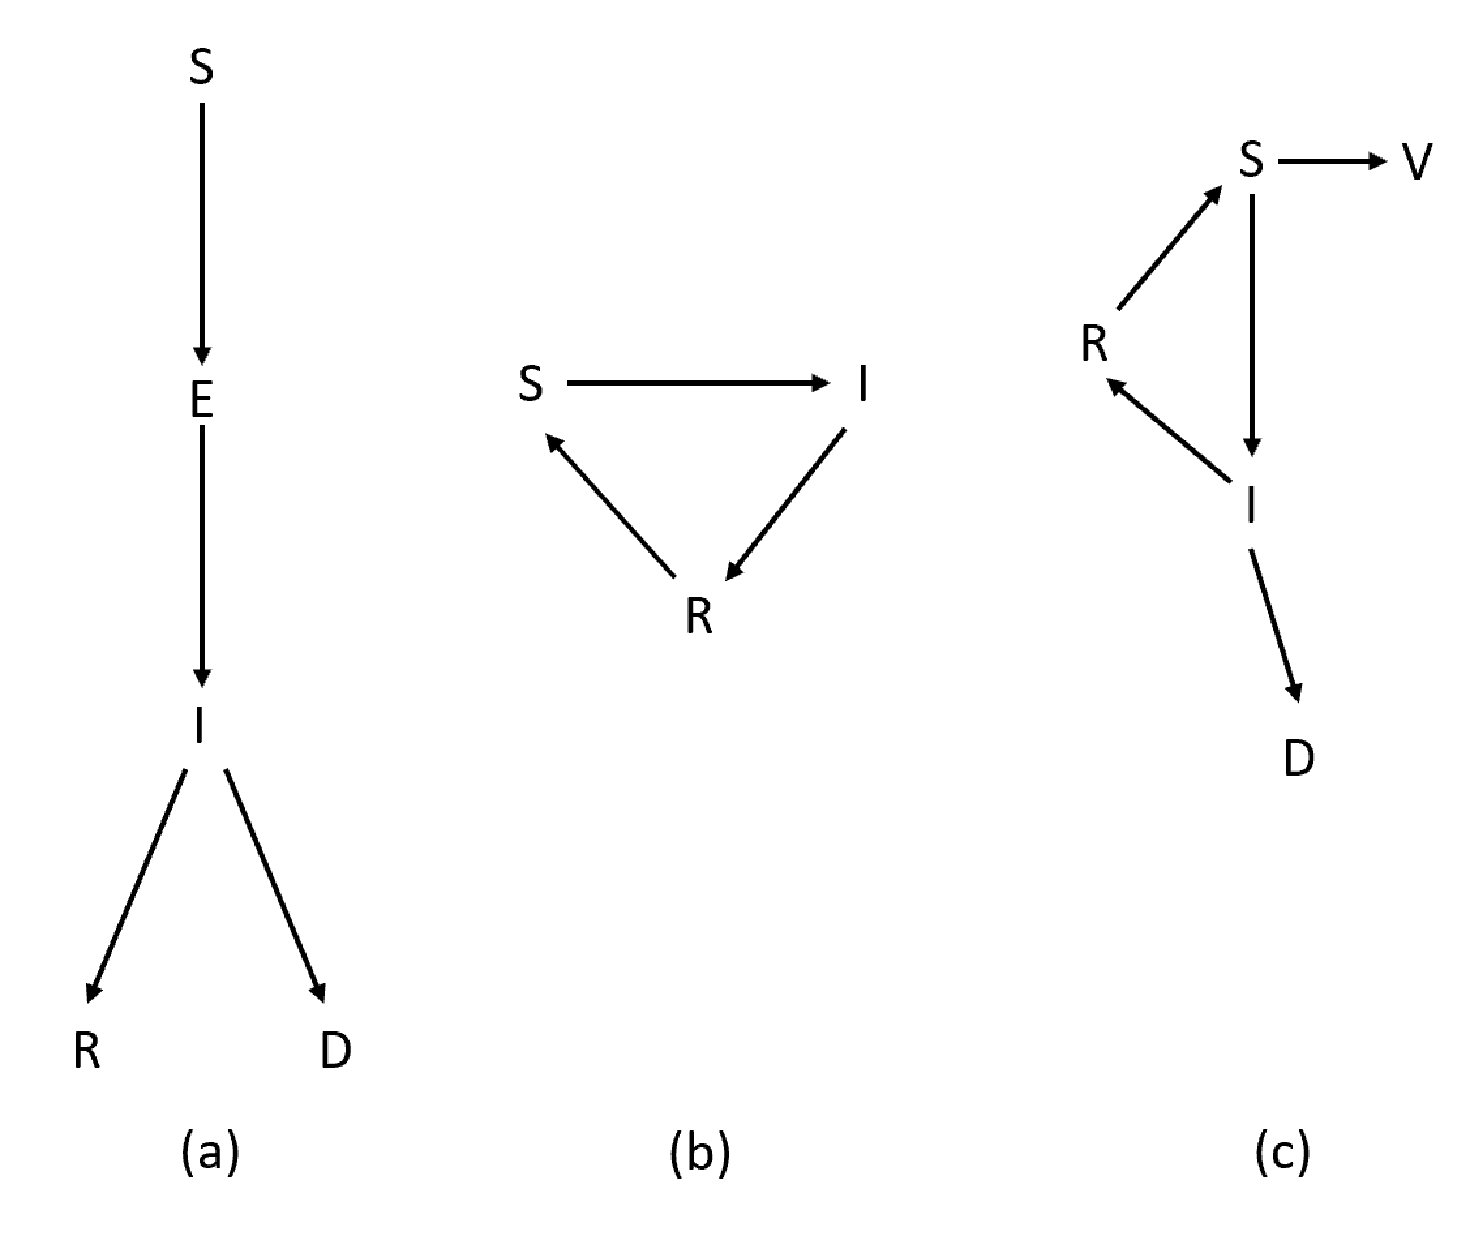
\includegraphics[width=0.6\linewidth]{latex/images/caus_eq2.pdf}
    % 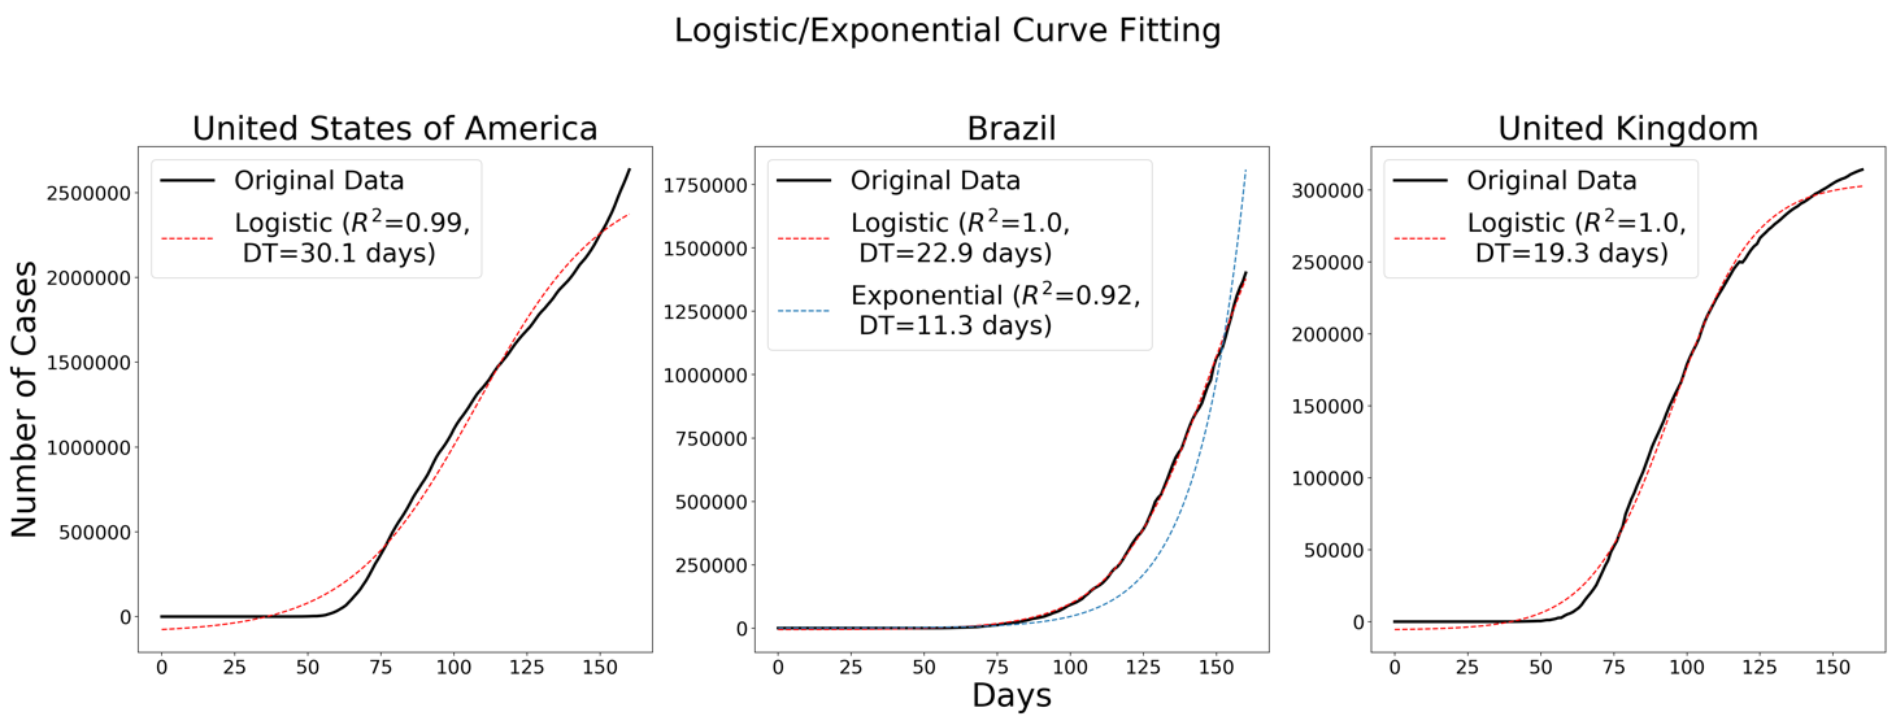
\includegraphics[width=15.5cm]{latex/images/fitting.PNG}%
    \caption{Advanced Models}
    \label{cd12}
\end{figure}

\clearpage

\section{Population Modelling Pseudo-code}
\label{code_alg}

\begin{algorithm}
\caption{Population Modelling Pseudo-code Outline}
\label{alg1}
% \vspace*{-.5cm}
% \begin{multicols}{2}
\begin{algorithmic}[1]
  \STATE $E \Leftarrow Contact\:Radius$
  \STATE $\overline{p} \Leftarrow Unlikeliness\:of\:Spread$
  \STATE $p\_died \Leftarrow Death\:Probability\:dependent\:on\:age$
  \FOR{$day\:in\:simulation\:days$}
  \FOR{$individual\:in\:population$}
      \STATE$Record\:individual\:status$
      \IF{$Infected$}
      \IF{$Draw\:with\:probability\:(p\_died\times age == 1)$}
        \STATE $individual\:status \Leftarrow Dead$
      \ELSE
        \IF{$(Rehabilitation\:days == 14)$}
          \STATE $individual\:status \Leftarrow Recovered$
        \ENDIF
        \STATE $Rehabilitation\:days\:+= 1$
      \ENDIF
      \ELSIF{$Susceptible$}
        \STATE $close\_people = 0$
        \FOR{$friend\:in\:community$}
        \IF{$(Friend==Infected)\:and\:(Euclid\:Dist<E)$}
        \STATE $close\_people\:+= 1$
        \ENDIF
        \ENDFOR
        \IF{$(Draw\:with\:probability\:dependent\:on\:close\_people\:and\:\overline{p} == 1)$}
          \STATE $individual\:status \Leftarrow Infected$
        \ENDIF
      \ENDIF
      \IF{$(Static == False)$}
          \STATE $individual\:X\:and\:Y\:position\:update$
          \IF{$individual\:X\:or\:Y\:position\:out\:of\:boundaries$}
            \STATE $Adjust\:position\:and\:reverse\:movement\:direction$
          \ENDIF
      \ENDIF
  \ENDFOR
\ENDFOR
\end{algorithmic}
% \end{multicols}
% \vspace*{-.4cm}
\end{algorithm}

\clearpage

\section{Clinical trials}
\label{ab_trials}
Making use of the data from the United States ClinicalTrials.gov website, it has been possible to gain insights about current clinical trials as of July 2020 against COVID-19 \cite{trials_data}. As can be seen from Figure \ref{trials}, Hydroxychloroquine has been so far the most common treatment tried.
\vspace{-0.2cm}
\begin{figure}[ht!]%
    \centering
    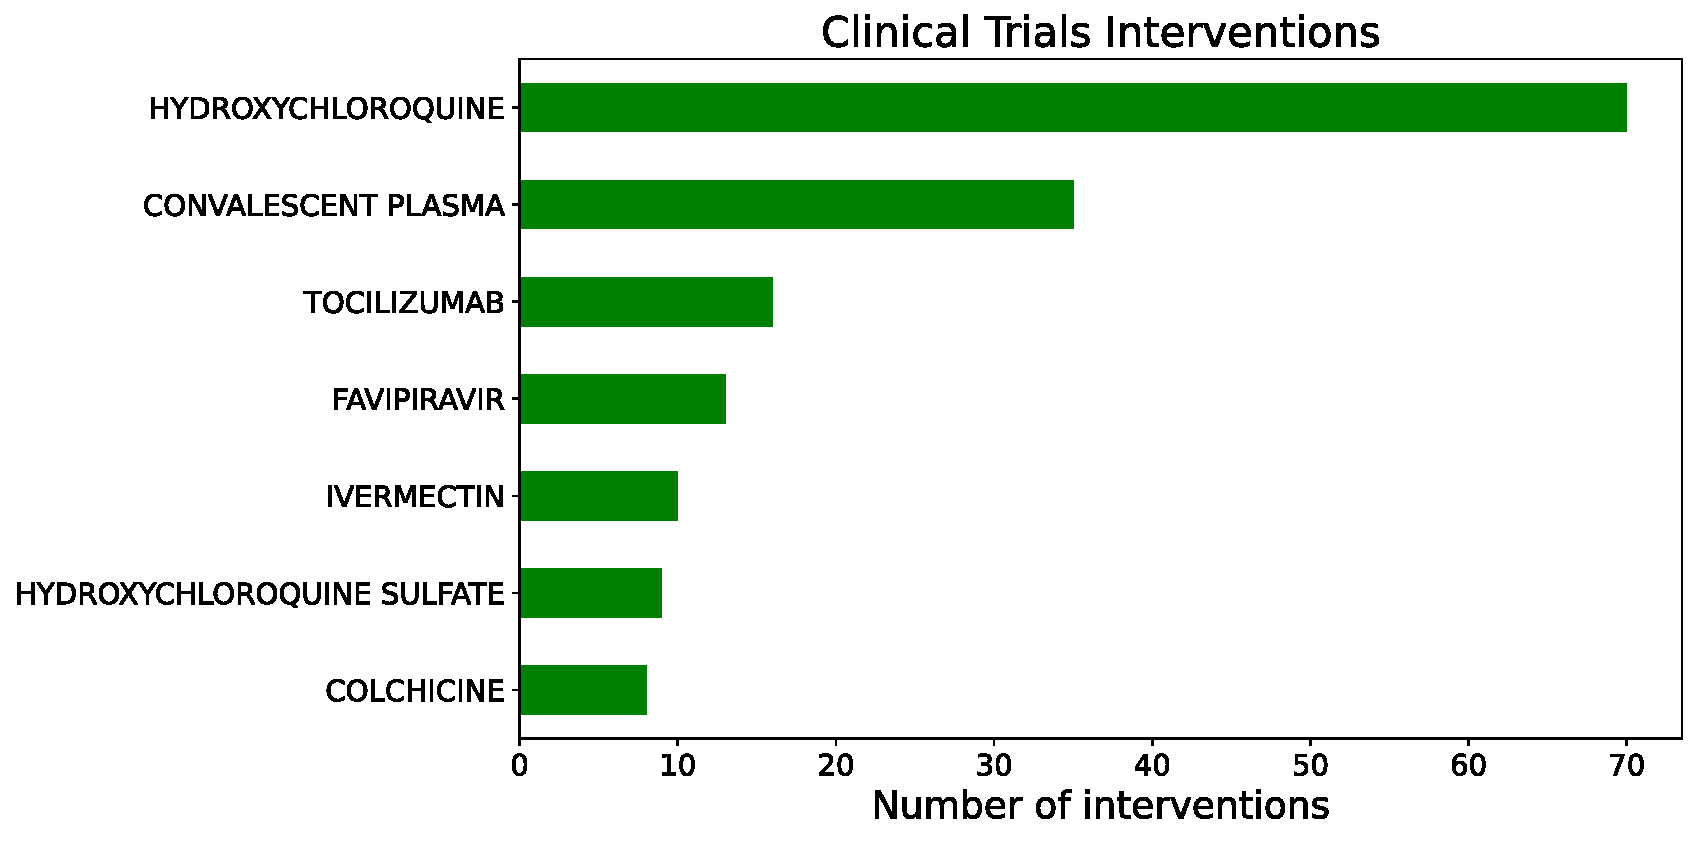
\includegraphics[width=0.65\linewidth]{latex/images/trials.pdf}
    % 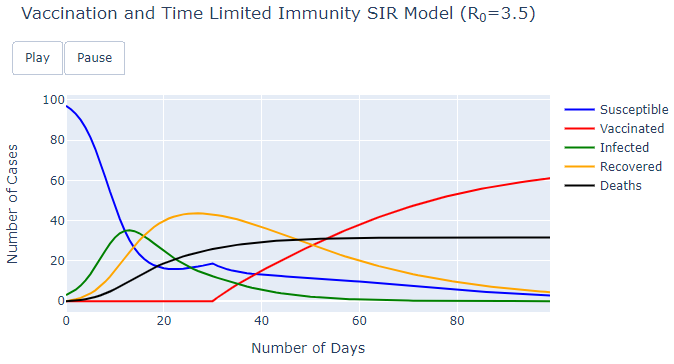
\includegraphics[width=13cm]{latex/images/vacc.PNG}%
    \vspace{-0.2cm}
    \caption{COVID-19 Clinical Trials}
    \label{trials}
\end{figure}
\vspace{-0.2cm}

As outlined in Section \ref{testing}, clinical trials are one of the main examples of A/B testing application. Gathering results from an A/B test, we can then be able to infer causal relationships about what can be the potential effects of a treatment \cite{power}.

In this setting, the Causal question we are asking ourselves is: Does a certain treatment decrease COVID-19 mortality rate? This question can then be formulated in statistical terms as a \textbf{null and alternative hypothesis}. In the null hypothesis, applying the treatment would not lead to any major change in the mortality rate and therefore both the treatment and control groups will be quite similar. Instead, in the alternative hypothesis, the treatment would cause a statistically significant change between the two groups. 

In our case, patients affected by COVID-19 would be considered as our population and our intervention (providing experimental medical treatment), would then be compared to no intervention. Variation in mortality rate could then be used as our metrics to asses the results. Patients should then be randomly assigned to either groups so that to avoid introduction of any form of bias (e.g. patients age, comorbidities, geographical location). If bias is unconsciously introduced, then this could lead to some form of \textbf{confounding bias}, which would then make it really difficult to disentangle what are effects due to the intervention and which ones are instead caused by a flaw in the randomization process. 

Following on with our example, the number of times an intervention leads to a substantial difference compared to the control group can then be summarised over a number of trials as a Binomial Distribution. In this distribution, the X axis will represent the count of possible outcomes, while the Y axis will represent the probability associated with an outcome. Although, according to the Central Limit Theorem, as we would increase our sample size, we would then end up with a Gaussian Distribution for each group in the experiment. 

In Figure \ref{test_dist}, there is shown a possible outcome for our example. As can be seen from the diagram, four different areas are present: True Positive (TP), True Negative (TN), False Positive (FP), False Negative (FN).
\vspace{-0.2cm}
\begin{figure}[ht!]%
    \centering
    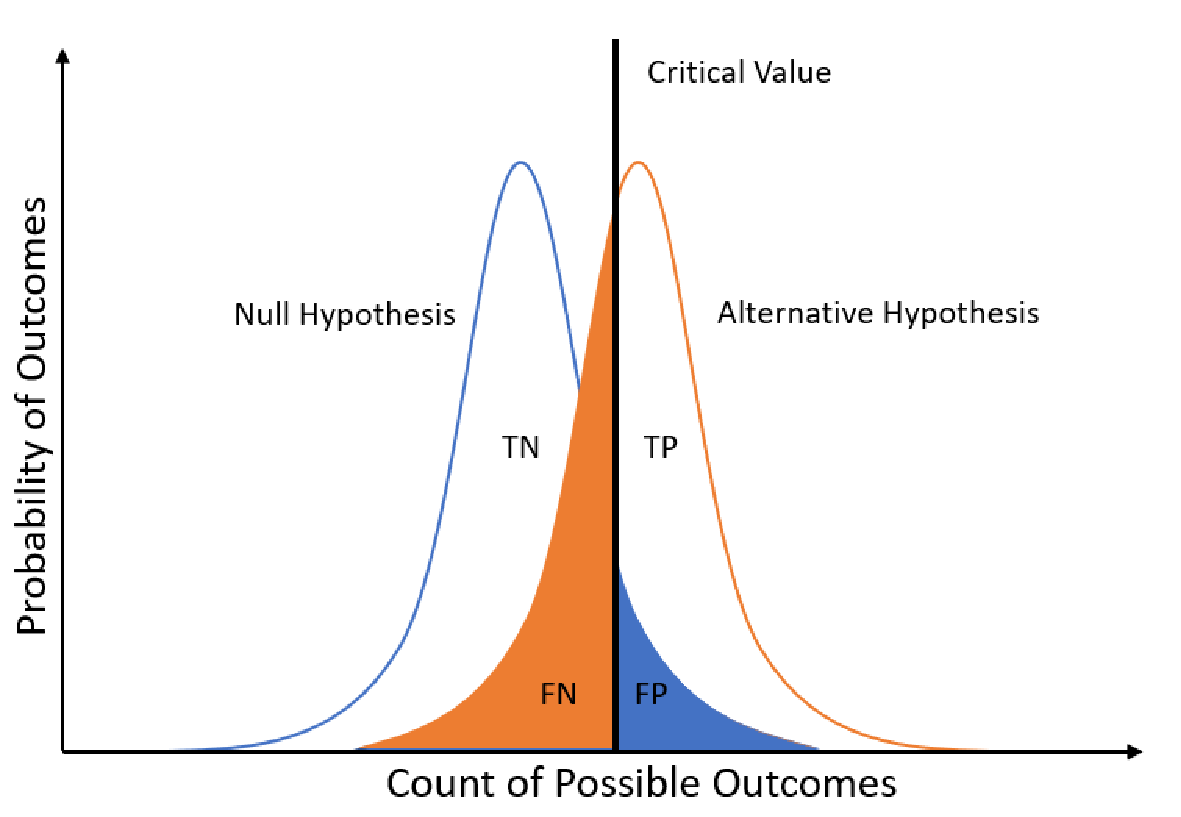
\includegraphics[width=0.6\linewidth]{latex/images/abtest.pdf}
    % 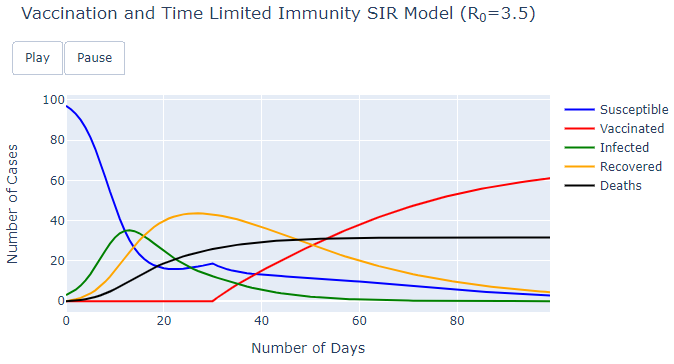
\includegraphics[width=13cm]{latex/images/vacc.PNG}%
    \vspace{-0.2cm}
    \caption{A/B Test Distributions}
    \label{test_dist}
\end{figure}
\vspace{-0.6cm}

In the TP case, we can affirm our treatment is beneficial since it managed to pass our test for the hypothesis (e.g. decreasing the mortality rate). In the case of the TN area, we can instead be confident that our treatment is not beneficial. While in the FP area, we might be deceived to believe our intervention was beneficial while it wasn't (the opposite holds true instead in the FN area). In these last two cases, it is then vital to look for any possible form of bias interference.

\clearpage
\section{Project Repository}
\label{repo}
Throughout this project, a private GitHub repository has been used as a key version control tool. The overall project has been structured into 4 different branches:

\begin{itemize}
    \item \textbf{Master:} In this branch, all the code and support files necessary in order to create the web application outlined in Chapter \ref{ch:progress} have been stored. The web application has been mainly developed on a local machine and then deployed on an Amazon Web Services EC2 Instance through Git control.  
    \item \textbf{Extras:} In this section there has instead been developed different parts of this project such as the code used to explain the Simpson Paradox (Section \ref{simp_ref}), Coronavirus comorbidities (Section \ref{como_app}), Survival Analysis (Section \ref{surv_app}), Power Predictive Score (Appendix \ref{pps}),  Clinical trials (Appendix \ref{ab_trials}). Additionally, for the SIR Time Series Estimation model introduced in Section \ref{tool_ref_app}, the has also been created an additional set-up in order to make possible to run this model easily through the command line.
    \item \textbf{Gh-pages:} This branch has instead been used to create and deploy through GitHub Pages a support website. This website has then been used to share two online presentations about the project (for the second examiner demonstration) and to create two online interactive shareable code notebook in order to explain how different aspects of the project have been programmed (Appendix \ref{dem}).  
    \item \textbf{Thesis:} This project report has been entirely created using \LaTeX\:    and synchronised with this branch of the repository in order to keep a backup and version control of the writing itself.
\end{itemize}

Additionally, a Wiki page has been included as part of the repository documentation in order to provide adequate background reading and context in case this project is going to be developed any further in the future (Figure \ref{wiki_ref}).
\\
\\
\begin{figure}[ht!]%
    \centering
    
\includegraphics[page=1,scale=0.56]{latex/images/wiki_page.pdf}
    \caption{Repository Wikipedia}%
    \label{wiki_ref}
\end{figure}
\\
\\
Finally, Github Actions have been included in order to add some form of Continuous Integration (CI) support in line with common DevOps (Development-Operations) principles.

\clearpage

\includepdf[pages=-,pagecommand=\section{Project Brief}\label{brief},noautoscale=true,offset=0 -70, scale=1.1]{latex/images/Outline.pdf}

\clearpage
\section{Design Archive Guide}
\label{archive}
A tree representation of the Project Design Archive is represented in the figure below. This image has been created through the windows command prompt using the tree command in the designed directory.
% \vspace*{-17mm}
% \setcounter{figure}{0}
\begin{figure}[ht!]%
    \centering
    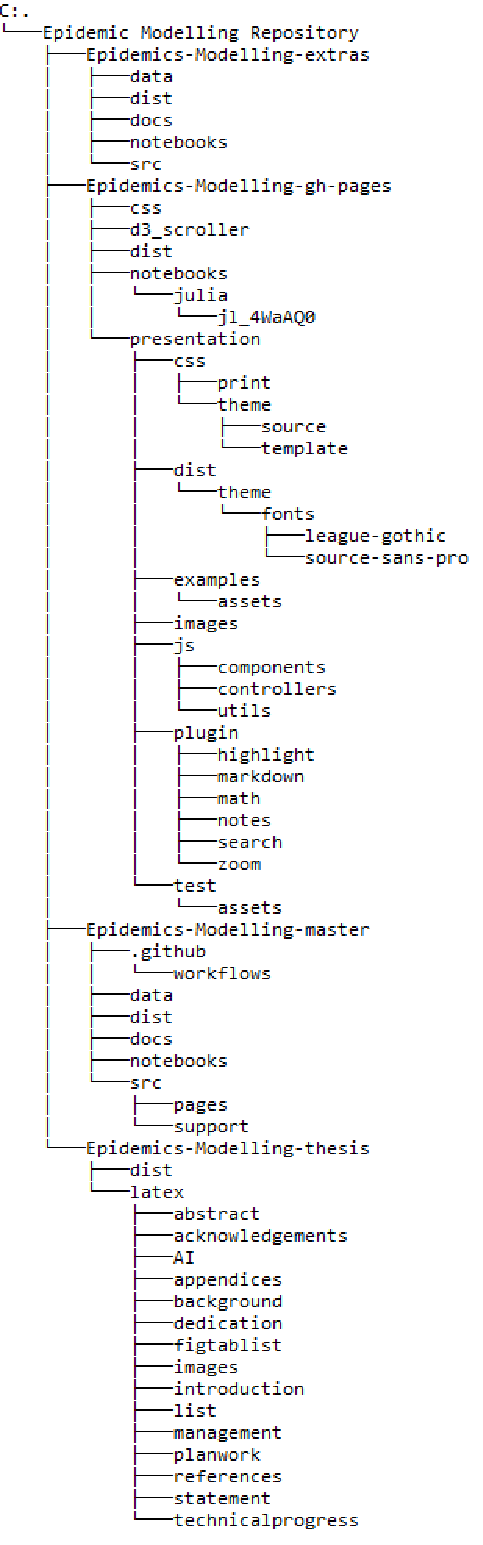
\includegraphics[page=1,scale=0.76]{latex/images/archive.pdf}
    \vspace*{-2mm}
    \caption{Design Archive}%
\end{figure}

\clearpage


\section{Word Count}
\label{count}

The registered word count for this report, starting from Chapter 1 to Chapter 6, was equal to 14,999 words. This has been measured using Doc Word Counter \cite{count_w}.

\end{appendices}